\section{疑难杂症} \label{sec:troubleshooting}

\subsection{出现字体缺失的编译失败提示}

一般情况下,如果你在编译“毕业设计论文”模板时出现了类似下面的编译报错:

\begin{minted}[frame=single]{bash}
  Package fontspec Error: The font "STXihei" cannot be found. ...
\end{minted}

这是由于你的电脑中尚未安装“华文细黑”这一字体,或你的电脑上安装的“华文细黑”字体文件名称不是 \texttt{STXIHEI.TTF},导致 {\LaTeX} 编译器找不到这一字体,也就导致无法正常编译模板。(毕业论文模板的封面中,中文标题要求字体为“华文细黑”。)

你可以通过下面的方法对这一问题进行排查。首先,在终端中运行:

\begin{minted}[frame=single]{bash}
  fc-list :lang-zh > fclist.txt
\end{minted}

这一命令会将你系统中安装的字体全部列出并保存在你执行命令所在目录下的 \texttt{fclist.txt} 文件中,你可以用文本编辑器打开这一文件,全局搜索“华文细黑”:

\begin{figure}[H]
  \centering
  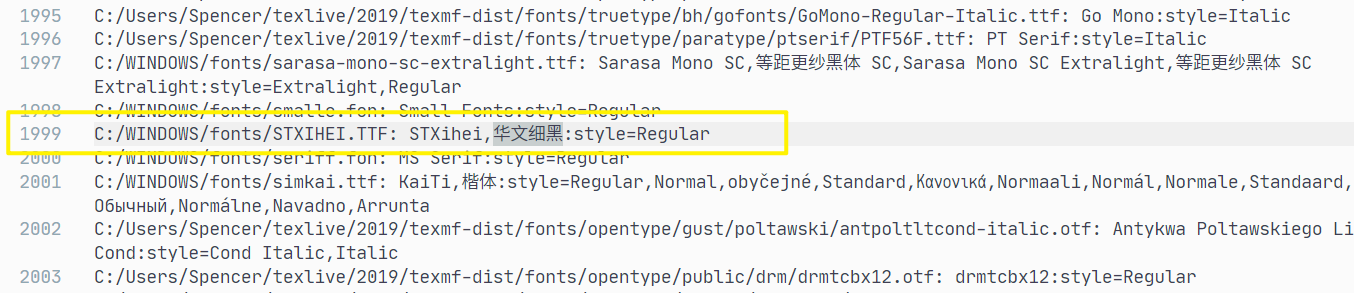
\includegraphics[width=\textwidth]{images/search_font.png}
  \caption{字体搜索}
  \label{search_font}
\end{figure}

如果你发现自己系统中并没有这一字体,需要手动安装,那么你需要确保安装之后字体文件的名称为 \texttt{STXIHEI.TTF}。你可以在 Windows 的\\ \texttt{C:\textbackslash\textbackslash Windows\textbackslash\textbackslash Fonts} 目录下找到你系统全局安装的字体,找到“华文细黑”并“右键 » 属性”,确认如下图所示:

\begin{figure}[H]
  \centering
  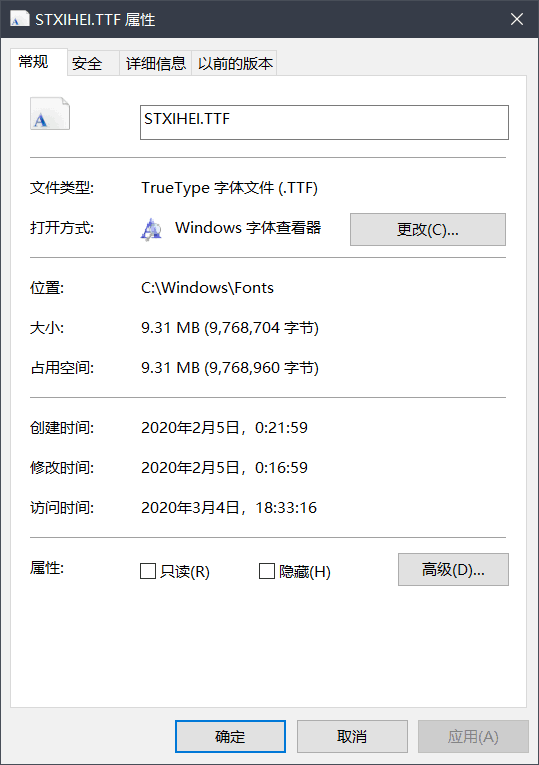
\includegraphics[width=0.6\textwidth]{images/font_property.png}
  \caption{字体属性}
  \label{font_property}
\end{figure}

之后,重启电脑,刷新字体缓存,确认编译状况。

如果 {\LaTeX} 编译器依旧找不到相关字体,我推荐重新安装 Windows 系统,或者将定义“华文细黑”字体的地方(毕业论文模板 \texttt{main.tex} 第 61 行至 63 行)与使用“华文细黑”字体的地方(毕业论文模板 \texttt{misc/0\_cover.tex} 第 43 行)删除,用默认字体替代。

\subsection{出现参考文献样式找不到的编译失败提示}

开题报告与毕业论文的参考文献均使用了 \href{https://github.com/hushidong/biblatex-gb7714-2015}{\color{RoyalBlue}{biblatex-gb7714-2015}} 宏包生成符合《GB/T 7714-2015 信息与文献 参考文献著录规则》规定的参考文献。这一参考文献宏包仅适用于最新版本的 \TeX Live 发行版(\TeX Live 2019)。如果你在编译过程中出现了类似如下的报错:

\begin{minted}[frame=single]{bash}
  Error: Style 'gb7714-2015' not found.
\end{minted}

那么就是由于你的 \TeX Live 发行版中没有包含这一宏包。需要你手动将 \TeX Live 更新为 2019 版本,或手动下载相应的宏包。(跨版本升级 \TeX Live 可能出现一些问题,推荐卸载重新安装。)

之后,在开始菜单中寻找 \TeX Live Manager,点击打开,并搜索\\ \texttt{biblatex-gb7714-2015},有如下输出表明你的宏包安装成功。

\begin{figure}[H]
  \centering
  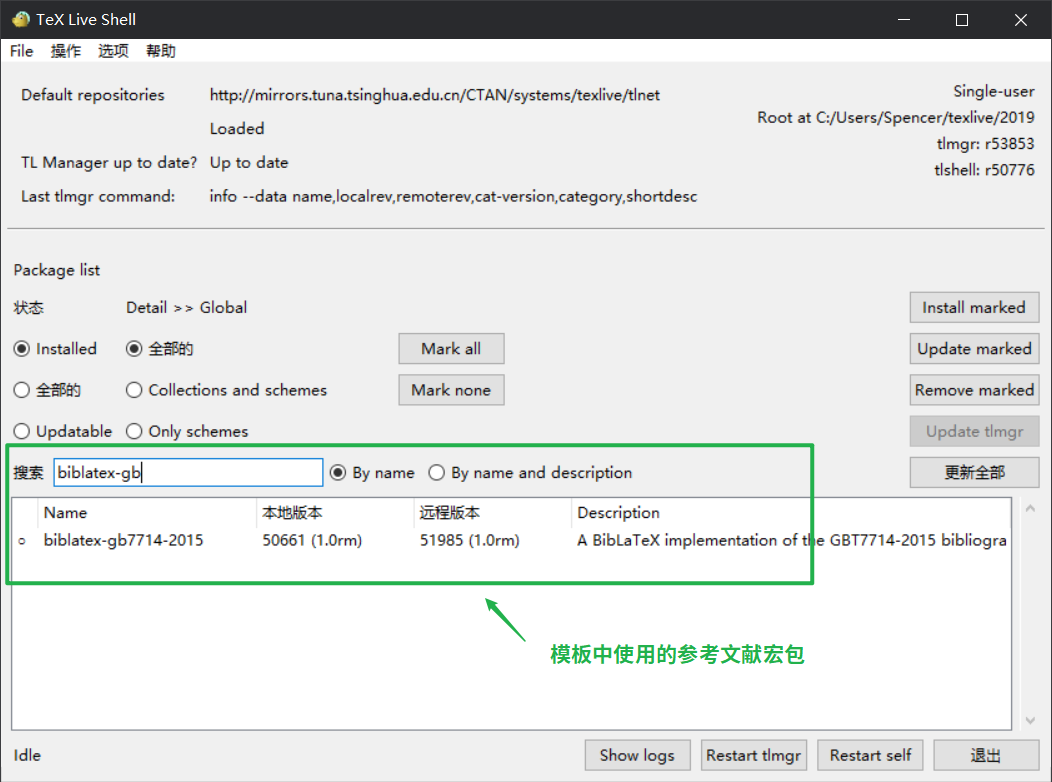
\includegraphics[width=\textwidth]{images/package_install_success.png}
  \caption{宏包安装成功}
  \label{package_install_success}
\end{figure}

\subsection{无法使用代码高亮 minted 宏包}

在论文中不可避免的要加入“代码块”。一般我们代码高亮使用的宏包都是 \texttt{minted},如果你发现插入 \texttt{minted} 环境后,编译失败,你可以尝试如下的方法解决:

\subsubsection{排查是否正确安装 Python 与 pygments 包}

如果你出现了类似如下的编译报错:

\begin{minted}[frame=single,linenos,breaklines]{bash}
  "Package minted Error: You must have `pygmentize' installed to use this package."
\end{minted}

那么是由于你的 Python 环境中缺少必要的库。\texttt{minted} 背后事实上用的是 Python 的 \texttt{pygments} 库进行代码渲染和高亮,因此你也必须安装 Python 环境和 \texttt{pygments} 库。你可以使用 Python 的官方包管理工具 pip 安装 \texttt{pygments}:

\begin{minted}[frame=single]{bash}
  pip install pygments
\end{minted}

之后,你需要确认可执行文件 \texttt{pygmentize.exe} 位于系统路径上。用如下的方法进行验证,如果出现类似输出,说明你的安装应该没有问题:

\begin{figure}[H]
  \centering
  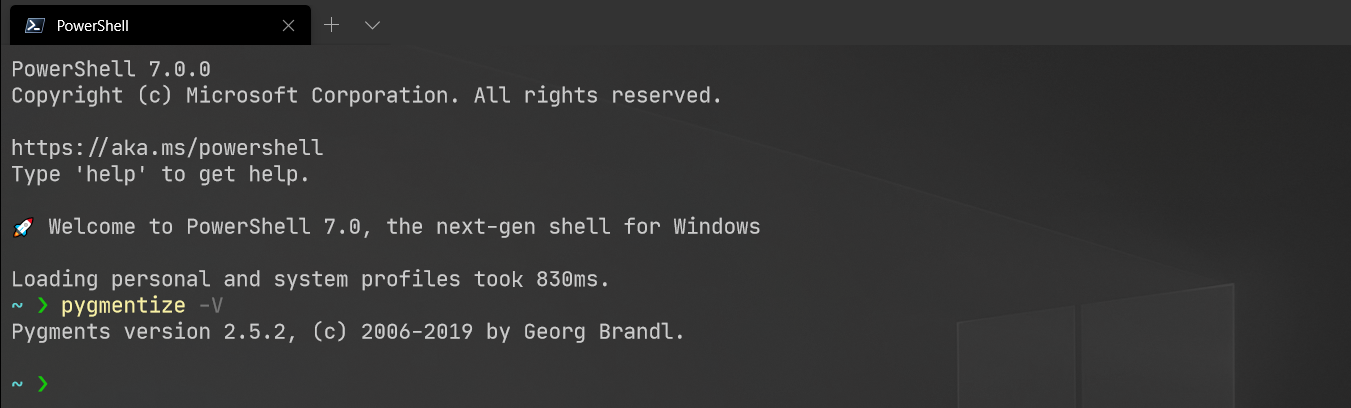
\includegraphics[width=\textwidth]{images/pygmentize_test.png}
  \caption{Pygmentize 安装成功}
  \label{pygmentize_test}
\end{figure}

\subsubsection{添加额外的编译参数}

如果你出现了类似如下的编译报错:

\begin{minted}[frame=single,linenos,breaklines]{bash}
  Package minted Error: You must invoke LaTeX with the -shell-escape flag.
\end{minted}

这是由于你的编译命令中没有添加 \texttt{-shell-escape} 参数,\texttt{minted} 宏包需要这一参数才能正确编译 {\LaTeX} 文档。以 VS Code 的 {\LaTeX} Workshop 为例,如果你使用 \texttt{xelatex} 编译,那么你需要将 \texttt{xelatex} 的编译参数修改如下:

\begin{minted}[frame=single]{json}
  {
    "name": "xelatex",
    "command": "xelatex",
    "args": [
        "-synctex=1",
        "-interaction=nonstopmode",
        "-file-line-error",
        "-pdf",
        "-shell-escape",
        "-outdir=%OUTDIR%",
        "-cd",
        "%DOC%"
    ],
    "env": {}
  }
\end{minted}

如果你使用 \texttt{latexmk} 编译,那么你需要将 \texttt{latexmk} 的编译参数修改如下:

\begin{minted}[frame=single]{json}
  {
    "name": "latexmk",
    "command": "latexmk",
    "args": [
        "-synctex=1",
        "-interaction=nonstopmode",
        "-file-line-error",
        "-xelatex",
        "-shell-escape",
        "-outdir=%OUTDIR%",
        "-cd",
        "%DOC%"
    ],
    "env": {}
  }
\end{minted}

\subsubsection{删除 minted 宏包的缓存文件夹}

如果你出现了类似如下的编译报错:
\begin{minted}[frame=single]{bash}
  ! Undefined control sequence.
\end{minted}

则可能是由于 \texttt{minted} 缓存导致。一般如果你编译过带有 \texttt{minted} 环境的 {\LaTeX} 项目,根目录都会有一个名称为 \texttt{\_minted\_doc} 的缓存文件夹。你可以尝试将这一文件夹删除,重新编译,排查问题。

\begin{figure}[H]
  \centering
  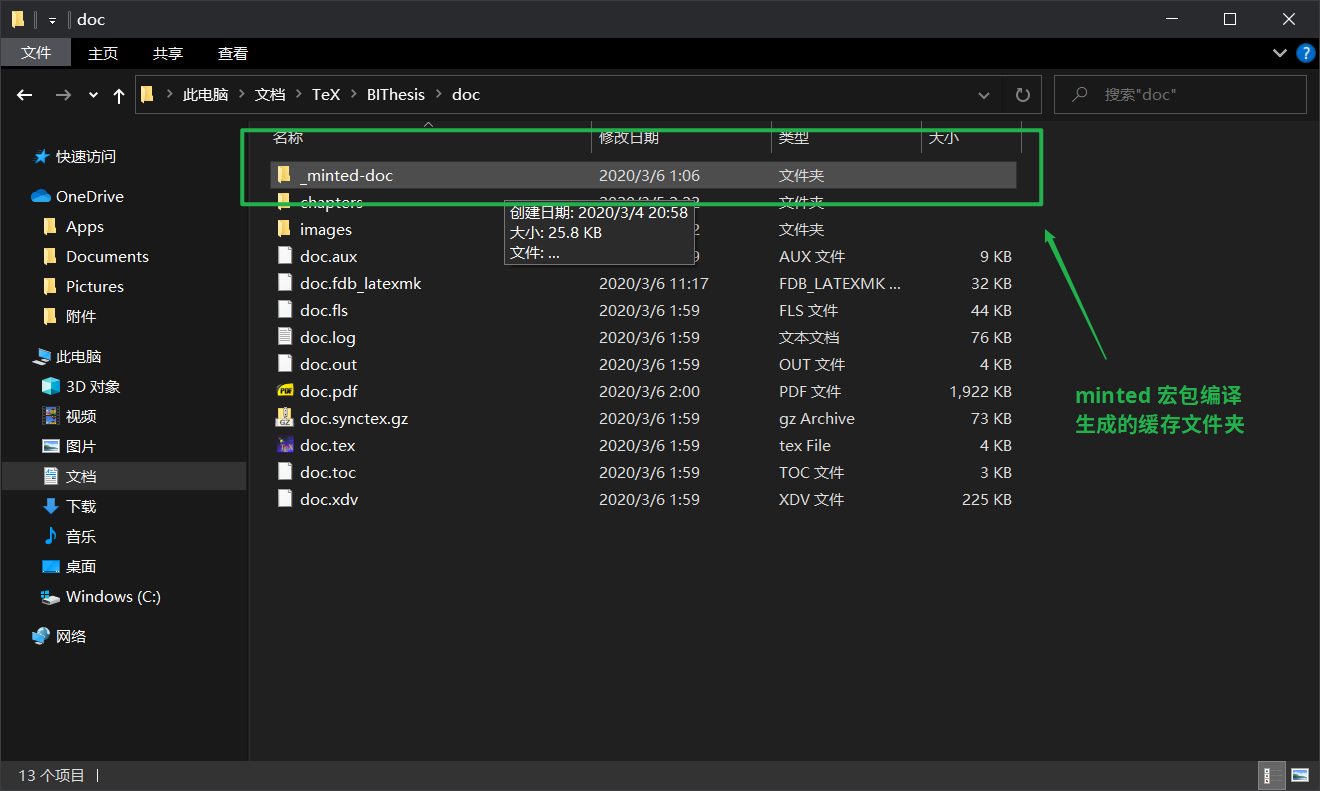
\includegraphics[width=\textwidth]{images/delete_minted_doc.png}
  \caption{删除 \texttt{\_minted-doc} 缓存文件夹}
  \label{delete_minted_doc}
\end{figure}

\subsection{编译过慢,一次更改需要编译半分钟}

如果你觉得模板中 \texttt{xelatex -> biber -> xelatex -> xelatex} 四步编译太慢,每次都全量编译,需要等待半分钟才能出结果,你可以尝试使用 \texttt{latexmk} 进行编译。\texttt{latexmk} 每次会根据你 {\LaTeX} 文档的更改,增量编译,从而加快对原文档进行微小变化后(比如只修改一个字)的编译速度。

另外,从我自己使用来看,\TeX studio 的编译速度一般都比 VS Code 快一些,如果你觉得 VS Code 的 LaTeX Workshop 编译太慢,可以考虑尝试使用 \TeX studio。
